../cictikz/src/cictikz/data/tex/cictikz_preamble.tex

% gm/ID against gate voltage, with the hand-calculation asymptotes.
%
% The point of the figure is that the two asymptotes the lecture derives
% bracket the real device and neither describes it in the middle, which is
% exactly where most designs sit. Weak inversion gives the flat ceiling
% 1/(n VT); strong inversion gives 2/Veff falling away to the right.
%
% Generated by py/tikzplot.py. Edit the script in ex/ that
% produced it and re-run that, not this file.

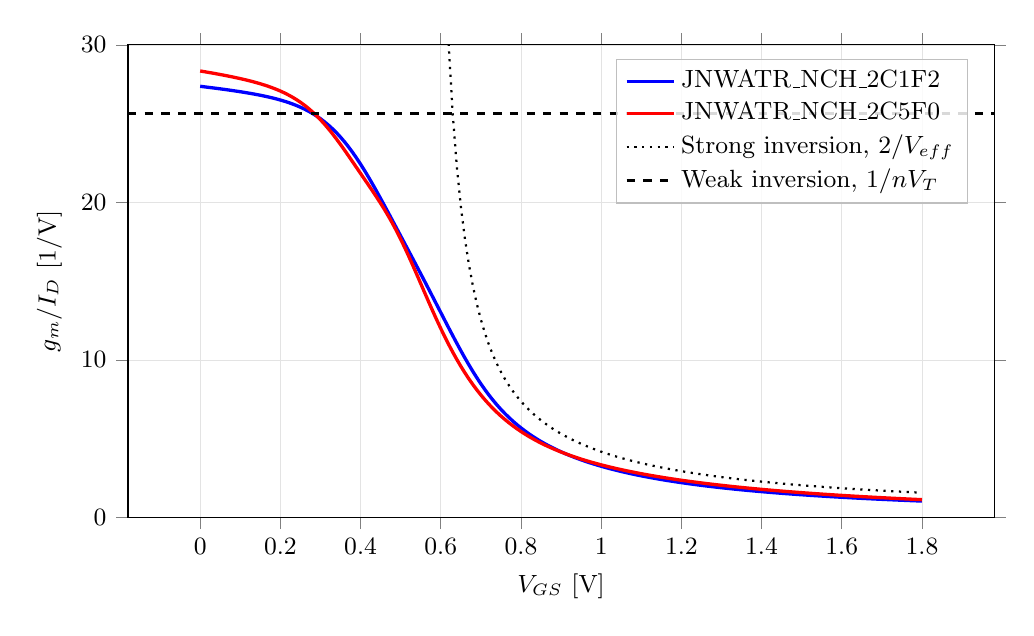
\begin{tikzpicture}[thick]

\begin{axis}[
  width=11.0cm,
  height=6.0cm,
  scale only axis,
  grid=both,
  grid style={gray!22, very thin},
  tick align=outside,
  tick label style={font=\small},
  label style={font=\small},
  title style={font=\small, yshift=-1mm},
  legend cell align=left,
  legend style={font=\small, draw=gray!50, fill=white, fill opacity=0.85, text opacity=1},
  xlabel={$V_{GS}$ [V]},
  ylabel={$g_m/I_D$ [1/V]},
  ymin=0,
  ymax=30,
  legend pos=north east
]
\addplot[blue, very thick, mark=none] coordinates {(0,27.373) (0.01,27.341) (0.02,27.309) (0.03,27.277) (0.04,27.244) (0.05,27.21) (0.06,27.176) (0.07,27.14) (0.08,27.104) (0.09,27.066) (0.1,27.027) (0.11,26.987) (0.12,26.944) (0.13,26.9) (0.14,26.853) (0.15,26.804) (0.16,26.751) (0.17,26.695) (0.18,26.635) (0.19,26.571) (0.2,26.501) (0.21,26.425) (0.22,26.343) (0.23,26.252) (0.24,26.154) (0.25,26.045) (0.26,25.925) (0.27,25.794) (0.28,25.649) (0.29,25.489) (0.3,25.313) (0.31,25.119) (0.32,24.906) (0.33,24.674) (0.34,24.42) (0.35,24.144) (0.36,23.845) (0.37,23.524) (0.38,23.18) (0.39,22.814) (0.4,22.427) (0.41,22.021) (0.42,21.597) (0.43,21.159) (0.44,20.707) (0.45,20.246) (0.46,19.778) (0.47,19.305) (0.48,18.828) (0.49,18.35) (0.5,17.872) (0.51,17.393) (0.52,16.913) (0.53,16.433) (0.54,15.951) (0.55,15.467) (0.56,14.98) (0.57,14.49) (0.58,13.997) (0.59,13.502) (0.6,13.007) (0.61,12.512) (0.62,12.02) (0.63,11.533) (0.64,11.054) (0.65,10.586) (0.66,10.131) (0.67,9.6907) (0.68,9.2679) (0.69,8.8637) (0.7,8.4791) (0.71,8.1148) (0.72,7.771) (0.73,7.4474) (0.74,7.1435) (0.75,6.8585) (0.76,6.5915) (0.77,6.3414) (0.78,6.1069) (0.79,5.8871) (0.8,5.6808) (0.81,5.4869) (0.82,5.3044) (0.83,5.1324) (0.84,4.9701) (0.85,4.8168) (0.86,4.6717) (0.87,4.5343) (0.88,4.404) (0.89,4.2802) (0.9,4.1626) (0.91,4.0507) (0.92,3.944) (0.93,3.8424) (0.94,3.7454) (0.95,3.6527) (0.96,3.564) (0.97,3.4792) (0.98,3.3979) (0.99,3.32) (1,3.2452) (1.01,3.1734) (1.02,3.1044) (1.03,3.0381) (1.04,2.9742) (1.05,2.9127) (1.06,2.8535) (1.07,2.7963) (1.08,2.7411) (1.09,2.6879) (1.1,2.6364) (1.11,2.5866) (1.12,2.5385) (1.13,2.492) (1.14,2.4469) (1.15,2.4032) (1.16,2.3609) (1.17,2.3198) (1.18,2.28) (1.19,2.2414) (1.2,2.2039) (1.21,2.1674) (1.22,2.132) (1.23,2.0976) (1.24,2.0641) (1.25,2.0316) (1.26,1.9999) (1.27,1.9691) (1.28,1.9391) (1.29,1.9098) (1.3,1.8813) (1.31,1.8536) (1.32,1.8265) (1.33,1.8001) (1.34,1.7744) (1.35,1.7492) (1.36,1.7247) (1.37,1.7008) (1.38,1.6774) (1.39,1.6546) (1.4,1.6323) (1.41,1.6105) (1.42,1.5892) (1.43,1.5684) (1.44,1.5481) (1.45,1.5282) (1.46,1.5087) (1.47,1.4896) (1.48,1.471) (1.49,1.4528) (1.5,1.4349) (1.51,1.4174) (1.52,1.4003) (1.53,1.3835) (1.54,1.3671) (1.55,1.351) (1.56,1.3352) (1.57,1.3197) (1.58,1.3046) (1.59,1.2897) (1.6,1.2751) (1.61,1.2608) (1.62,1.2468) (1.63,1.2331) (1.64,1.2196) (1.65,1.2063) (1.66,1.1933) (1.67,1.1805) (1.68,1.168) (1.69,1.1557) (1.7,1.1436) (1.71,1.1318) (1.72,1.1201) (1.73,1.1086) (1.74,1.0974) (1.75,1.0863) (1.76,1.0755) (1.77,1.0648) (1.78,1.0543) (1.79,1.044) (1.8,1.0338)};
\addlegendentry{JNWATR\_NCH\_2C1F2}
\addplot[red, very thick, mark=none] coordinates {(0,28.345) (0.01,28.302) (0.02,28.258) (0.03,28.214) (0.04,28.168) (0.05,28.121) (0.06,28.072) (0.07,28.022) (0.08,27.97) (0.09,27.916) (0.1,27.86) (0.11,27.802) (0.12,27.74) (0.13,27.675) (0.14,27.606) (0.15,27.532) (0.16,27.453) (0.17,27.369) (0.18,27.277) (0.19,27.178) (0.2,27.07) (0.21,26.953) (0.22,26.824) (0.23,26.683) (0.24,26.529) (0.25,26.359) (0.26,26.174) (0.27,25.971) (0.28,25.75) (0.29,25.509) (0.3,25.249) (0.31,24.97) (0.32,24.671) (0.33,24.355) (0.34,24.022) (0.35,23.676) (0.36,23.319) (0.37,22.953) (0.38,22.583) (0.39,22.211) (0.4,21.838) (0.41,21.466) (0.42,21.093) (0.43,20.717) (0.44,20.334) (0.45,19.941) (0.46,19.532) (0.47,19.103) (0.48,18.65) (0.49,18.171) (0.5,17.666) (0.51,17.136) (0.52,16.585) (0.53,16.016) (0.54,15.435) (0.55,14.847) (0.56,14.258) (0.57,13.674) (0.58,13.099) (0.59,12.538) (0.6,11.993) (0.61,11.468) (0.62,10.965) (0.63,10.485) (0.64,10.028) (0.65,9.5947) (0.66,9.1852) (0.67,8.7989) (0.68,8.4351) (0.69,8.0929) (0.7,7.7713) (0.71,7.4692) (0.72,7.1856) (0.73,6.9192) (0.74,6.6691) (0.75,6.4342) (0.76,6.2133) (0.77,6.0056) (0.78,5.8101) (0.79,5.6259) (0.8,5.4522) (0.81,5.2883) (0.82,5.1333) (0.83,4.9868) (0.84,4.848) (0.85,4.7165) (0.86,4.5916) (0.87,4.4729) (0.88,4.36) (0.89,4.2524) (0.9,4.1498) (0.91,4.0519) (0.92,3.9583) (0.93,3.8687) (0.94,3.7829) (0.95,3.7007) (0.96,3.6217) (0.97,3.5459) (0.98,3.473) (0.99,3.4028) (1,3.3351) (1.01,3.2699) (1.02,3.207) (1.03,3.1463) (1.04,3.0876) (1.05,3.0309) (1.06,2.9759) (1.07,2.9227) (1.08,2.8712) (1.09,2.8213) (1.1,2.7728) (1.11,2.7258) (1.12,2.6801) (1.13,2.6357) (1.14,2.5926) (1.15,2.5506) (1.16,2.5098) (1.17,2.4701) (1.18,2.4314) (1.19,2.3937) (1.2,2.357) (1.21,2.3212) (1.22,2.2863) (1.23,2.2522) (1.24,2.219) (1.25,2.1866) (1.26,2.1549) (1.27,2.1239) (1.28,2.0937) (1.29,2.0642) (1.3,2.0353) (1.31,2.007) (1.32,1.9794) (1.33,1.9524) (1.34,1.9259) (1.35,1.9) (1.36,1.8747) (1.37,1.8499) (1.38,1.8256) (1.39,1.8018) (1.4,1.7784) (1.41,1.7556) (1.42,1.7332) (1.43,1.7112) (1.44,1.6897) (1.45,1.6686) (1.46,1.6478) (1.47,1.6275) (1.48,1.6076) (1.49,1.588) (1.5,1.5688) (1.51,1.55) (1.52,1.5315) (1.53,1.5133) (1.54,1.4955) (1.55,1.478) (1.56,1.4607) (1.57,1.4438) (1.58,1.4272) (1.59,1.4109) (1.6,1.3949) (1.61,1.3791) (1.62,1.3636) (1.63,1.3483) (1.64,1.3334) (1.65,1.3186) (1.66,1.3041) (1.67,1.2899) (1.68,1.2759) (1.69,1.2621) (1.7,1.2485) (1.71,1.2352) (1.72,1.222) (1.73,1.2091) (1.74,1.1964) (1.75,1.1838) (1.76,1.1715) (1.77,1.1594) (1.78,1.1474) (1.79,1.1356) (1.8,1.1241)};
\addlegendentry{JNWATR\_NCH\_2C5F0}
\addplot[black, dotted, thick, mark=none] coordinates {(0.61,35.978) (0.62,29.903) (0.63,25.557) (0.64,22.297) (0.65,19.761) (0.66,17.735) (0.67,16.081) (0.68,14.707) (0.69,13.548) (0.7,12.56) (0.71,11.709) (0.72,10.969) (0.73,10.321) (0.74,9.7491) (0.75,9.241) (0.76,8.7869) (0.77,8.3788) (0.78,8.0098) (0.79,7.6746) (0.8,7.3687) (0.81,7.0881) (0.82,6.8295) (0.83,6.5905) (0.84,6.3686) (0.85,6.162) (0.86,5.9692) (0.87,5.7886) (0.88,5.6191) (0.89,5.4597) (0.9,5.3094) (0.91,5.1674) (0.92,5.0332) (0.93,4.9059) (0.94,4.7851) (0.95,4.6703) (0.96,4.5611) (0.97,4.457) (0.98,4.3576) (0.99,4.2627) (1,4.172) (1.01,4.0851) (1.02,4.0018) (1.03,3.922) (1.04,3.8454) (1.05,3.7717) (1.06,3.7009) (1.07,3.6328) (1.08,3.5671) (1.09,3.5039) (1.1,3.4429) (1.11,3.384) (1.12,3.3272) (1.13,3.2722) (1.14,3.2191) (1.15,3.1677) (1.16,3.118) (1.17,3.0698) (1.18,3.0231) (1.19,2.9779) (1.2,2.934) (1.21,2.8913) (1.22,2.85) (1.23,2.8098) (1.24,2.7708) (1.25,2.7328) (1.26,2.6959) (1.27,2.66) (1.28,2.6251) (1.29,2.591) (1.3,2.5579) (1.31,2.5256) (1.32,2.4941) (1.33,2.4634) (1.34,2.4335) (1.35,2.4043) (1.36,2.3758) (1.37,2.348) (1.38,2.3208) (1.39,2.2943) (1.4,2.2684) (1.41,2.243) (1.42,2.2183) (1.43,2.1941) (1.44,2.1704) (1.45,2.1472) (1.46,2.1245) (1.47,2.1023) (1.48,2.0806) (1.49,2.0593) (1.5,2.0385) (1.51,2.0181) (1.52,1.9981) (1.53,1.9785) (1.54,1.9592) (1.55,1.9404) (1.56,1.9219) (1.57,1.9038) (1.58,1.886) (1.59,1.8686) (1.6,1.8515) (1.61,1.8347) (1.62,1.8182) (1.63,1.802) (1.64,1.786) (1.65,1.7704) (1.66,1.7551) (1.67,1.74) (1.68,1.7252) (1.69,1.7106) (1.7,1.6963) (1.71,1.6822) (1.72,1.6684) (1.73,1.6547) (1.74,1.6414) (1.75,1.6282) (1.76,1.6152) (1.77,1.6025) (1.78,1.5899) (1.79,1.5776) (1.8,1.5654)};
\addlegendentry{Strong inversion, $2/V_{eff}$}
\addlegendimage{black, dashed, thick}
\addlegendentry{Weak inversion, $1/nV_T$}
\draw[black, dashed, thick] ({rel axis cs:0,0} |- {axis cs:0,25.641}) -- ({rel axis cs:1,0} |- {axis cs:0,25.641});
\end{axis}

\end{tikzpicture}
\end{document}
